\documentclass[generalized_symmetry.tex]{subfiles}
\setcounter{chapter}{3}
\begin{document}

\chapter{高次形式対称性}
これまでは主に2次元の一般化対称性について見てきましたが、ここから徐々に高次元の一般化対称性について見ていくことにします。まずは、高次元での高次形式対称性と呼ばれるクラスの一般化対称性について見ていきます。

\section{高次形式対称性の定義}

まず$p$形式対称性を定義します。群$G$があって、$g\in G$と時空内の余次元$p+1$の向きのついた面$M$があったときに$M$に局在したトポロジカル欠陥$U_g(M)$が存在して、次の条件を満たすとき、これを$p$形式対称性と呼びます。
\begin{enumerate}
    \item フュージョン則は群の積になります。
    \begin{align}
        \orientedline{U_g}
        \orientedline{U_h}
        =
        \orientedline{U_{gh}}
    \end{align}
    \item 単位元、逆元も群の構造に従います。つまり
    \begin{align}
        U_1(M) = 1, \quad U_{g^{-1}}(M) = U_g(-M)
    \end{align}
    となります。
\end{enumerate}
この言葉遣いでは$0$形式対称性は普通の対称性です。$p>0$のとき$p$形式対称性は高次形式対称性と呼ばれます。高次形式対称性の場合には、トポロジカルな変形でフュージョンの順番を入れ替えることができるので、群$G$はアーベル群になります。

次に、$p$形式対称性の欠陥(演算子)への作用について見ていきましょう。一般に$p$形式対称性は$p$次元の欠陥に自然に作用します。例えば普通の対称性は$0$形式対称性ですから、$0$次元の欠陥である局所演算子に自然に作用します。もう少し正確に述べます。$C$を次元$p$の曲面として$W_a(C)$を$C$に局在した次元$p$の(トポロジカルとは限らない)欠陥とします。ここで$a$はラベルです。余次元$p+1$の曲面$M$を$C$に絡み数1で絡んでいる曲面として$U_g(M)$は$W_a(C)$に次のように作用します。
\begin{align}
    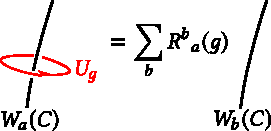
\includegraphics{actionp-formsym.pdf}.
\end{align}
ここで$R^{b}{}_{a}(g)$は$G$の表現行列です。高次形式対称性の場合には$G$はアーベル群でしたから、既約表現は1次元です。つまり、$R^{b}{}_{a}(g)=$(位相)$\delta^{b}_{a}$となる基底をとることができます。

いくつかコメントをします。
\begin{itemize}
    \item 高次形式対称性の最も代表的な例はゲージ理論の中心対称性です。これは次の節で格子ゲージ理論の場合に詳しく見ていきます。
    \item 実は高次形式対称性は様々な場面で知られていました。例えば弦理論において弦やブレーンが電荷を持つゲージ対称性は高次形式対称性です。格子ゲージ理論の中心対称性も閉じ込めと非閉じ込めを区別する対称性として格子ゲージ理論の文脈で知られていました。ただ、大域的高次形式を局所的なトポロジカル欠陥として理解し、様々な場の理論への応用への道を切り開いたのが\cite{Gaiotto:2014kfa}です。
\end{itemize}

\section{格子ゲージ理論の中心対称性}
ここでは高次形式対称性の例としてゲージ理論の中心対称性を紹介します。これは格子ゲージ理論の見方からすると対称性の見方①(変換で作用を不変にするもの)でも理解できるので、まずはそれを説明します。

\subsection{格子ゲージ理論}
格子ゲージ理論はすでに出てきましたが、ここで改めて説明します。ここでは問題を具体的にするためにゲージ群が$\SU(N)$の場合を考えますが、別のコンパクト群の場合でも同様に格子ゲージ理論を構成することができます。注意することは、格子ゲージ理論の場合にはLie代数ではなくて群をそのまま考えることです。$d$次元の超立方格子を考えます。ゲージ群は各リンク$\expval{ij}$に群の元$U_{ij}\in \SU(N)$を割り当てます。向きを反対にした場合の記号の使い方として$U_{ji}=U_{ij}^{-1}$とします。分配関数は
\begin{align}
    Z = \int \prod_{\expval{ij}: \text{すべてのリンク}} dU_{ij} \exp(-S[U_{ij}]),\nonumber\\
    S[U] = - K \sum_{\expval{ijkl}:\text{すべてのプラケット}}\left[ \Tr( U_{ij}U_{jk}U_{kl}U_{li})+(\text{複素共役})\right]
    \label{Wilsonaction}
\end{align}
と書けます。ここで$K$は定数で、ゲージ結合定数$g_{\mathrm{YM}}$と$K\sim 1/g_{\mathrm{YM}}^2$という形で関係しています。また積分$\int dU_{ij}$はHaar測度と呼ばれる積分測度で、群の元をかける作用で不変です。

格子ゲージ理論のゲージ対称性は次のように記述されます。ゲージ変換のパラメータは各頂点に割り当てられたゲージ群の元$g_i\in \SU(N)$です。ゲージ変換はリンクに次のように作用します。
\begin{align}
    U_{ij}' = g_i U_{ij} g_j^{-1}.
\end{align}
Haar測度と作用\eqref{Wilsonaction}はこの変換で不変です。

\subsection{格子ゲージ理論の中心対称性}

格子ゲージ理論の中心対称性を説明するために少し群についての準備をします。$\SU(N)$の元の中で単位行列に比例するような元を考えます。例えば$\omega=\exp(2\pi i/N)$として$\omega \mathbf{1}$は$\SU(N)$の元です。このような元をすべて集めてきた集合
\begin{align}
    \Zcal = \{ \omega^k \mathbf{1} | k=0,1,\dots,N-1 \}\subset \SU(N)
\end{align}
は$\SU(N)$のすべての元を可換な最大の部分群です\footnote{$\SU(N)$のすべての元と可換な元は単位行列に比例することは、Schurの補題から分かります。}。このような部分群を中心と呼びます。$\Zcal$は群として$\Zb_N$と同型です。

次に中心対称性を記述します。ここでは\ref{sec:symmetrydefect2}節で説明したのと同様のやり方で説明します。図\ref{fig:faceboundary}のように、立方格子の時空の中で余次元1の向きのついた面$M$を考えます。$M$はサイトを通らないことにします。$M$は境界を持っていて、その境界を$\Sigma=\del M$とします。$M$は余次元1でリンクを横切っていっていて、$\Sigma$は余次元2でプラケットの中を繋いでいっていることに注意してください。

\begin{figure}[htbp]
    \centering
    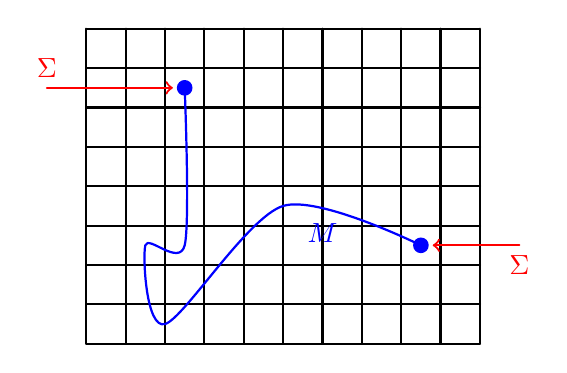
\begin{tikzpicture}[scale=1.0, line cap=round, line join=round]
        % グリッド((0,0) から (5,4) まで 1cm ごと)
        \draw[step=0.5cm, thick] (0,0) grid (5,4);
        
        % 青い経路と始点・終点
        \draw[blue, thick, smooth] plot coordinates {(1.25,3.25) (1.25, 1.25) (0.75,1.25) (1,0.25) (2.5,1.75) (4.25,1.25)};
        \draw[blue, thick] (1.25,3.25) node[fill=blue,circle,inner sep=2pt]{};
        \draw[blue, thick] (4.25,1.25) node[fill=blue,circle,inner sep=2pt] {};
        
        % 経路付近に “M” のラベル
        \node[blue] at (3,1.4) {$M$};
        
        % 赤い矢印とシグマの記号(上の矢印は右向き,下の矢印は左向き)
        \draw[<-, red, thick] (1.1,3.25) -- (-0.5,3.25) node[above] {$\Sigma$};
        \draw[<-, red, thick] (4.4,1.25) -- (5.5,1.25) node[below] {$\Sigma$};
    \end{tikzpicture}
    \caption{面$M$とその境界$\Sigma$}
    \label{fig:faceboundary}
\end{figure}

この上で次のような積分変数の変換をします。簡単のために中心$\Zcal$の元$\omega$に注目します。
\begin{align}
    U_{ij}'=
    \begin{cases}
        U_{ij} & \text{$\expval{ij}$が$\Sigma$を横切らない},\\
        \omega U_{ij} & \text{$\expval{ij}$が$\Sigma$正の方向に横切る}.
        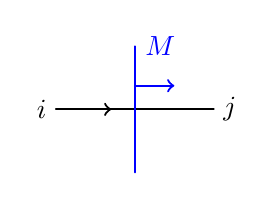
\begin{tikzpicture}[baseline=0pt, line cap=round, line join=round, scale=1]
            % 水平矢印(中心から右へ)
            \draw[->, thick] (0,0) -- (0.7,0);
            \draw[thick] (0,0) -- (2,0);
            \node[right] at (2,0) {$j$};        
            \node[left] at (0,0) {$i$};        
            % --- 青い縦線 ---
            % 下から上へ線
            \draw[blue, thick] (1,-0.8) -- (1,0.8)node[above,right]{$M$};
            % --- 上部の青い矢印(左→右)
            \draw[->, blue, thick] (1,0.3) -- (1.5,0.3);
            % --- “j” の文字ラベル ---
        \end{tikzpicture}
        \\
        \omega^{-1} U_{ij} & \text{$\expval{ij}$が$\Sigma$負の方向に横切る}.
        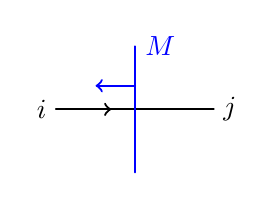
\begin{tikzpicture}[baseline=0pt, line cap=round, line join=round, scale=1]
            % 水平矢印(中心から右へ)
            \draw[->, thick] (0,0) -- (0.7,0);
            \draw[thick] (0,0) -- (2,0);
            \node[right] at (2,0) {$j$};        
            \node[left] at (0,0) {$i$};        
            % --- 青い縦線 ---
            % 下から上へ線
            \draw[blue, thick] (1,-0.8) -- (1,0.8)node[above,right]{$M$};
            % --- 上部の青い矢印(左→右)
            \draw[->, blue, thick] (1,0.3) -- (0.5,0.3);
            % --- “j” の文字ラベル ---
        \end{tikzpicture}
    \end{cases}
    \label{centergaugetrans}
\end{align}
複数回横切っている場合には、それらの操作をすべて行います。

この変換は次の性質を持ちます。まず、この変換は群の元をかけているだけなので、Haar測度は不変です。次に作用を考えます。作用は不変ではありませんが、どれくらい変化するかを考えます。作用はプラケットの和ですから、一つ一つのプラケットについて考えます。
\newcommand{\plaquette}{
  \draw[thick] (-1,-1) rectangle (1,1);
  \draw[->, thick] (-1,-1) -- (0,-1); % 下辺 → 右
  \draw[->, thick] (1,-1) -- (1,0);   % 右辺 → 上
  \draw[->, thick] (1,1) -- (0,1);  % 上辺 → 左
  \draw[->, thick] (-1,1) -- (-1,0);% 左辺 → 下
}
\begin{itemize}
    \item $M$と交わらないようなプラケットは変化しません。
    \begin{align}
        \begin{tikzpicture}[scale=0.5,baseline=0pt]
        \plaquette
        \end{tikzpicture}\ 
        =\ 
        \begin{tikzpicture}[scale=0.5,baseline=0pt]
        \plaquette
        \end{tikzpicture}
    \end{align}
    \item $M$と$\Sigma$以外のところで交わるプラケットを考えます。この場合、正の方向に交わるのと負の方向に交わるのが同じ回数だけあるので、結果として作用は変化しません。
    \begin{align}
        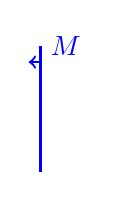
\begin{tikzpicture}[scale=0.5,baseline=0pt]
        \plaquette
        \draw[blue, thick] (0.6,-1.5) -- (0.6,1.7)node[above,right]{$M$};
        % --- 上部の青い矢印(左→右)
        \draw[->, blue, thick] (0.6,1.3) -- (0.3,1.3);
        \end{tikzpicture}\ 
        =\ 
        \begin{tikzpicture}[scale=0.5,baseline=0pt]
        \plaquette
        \end{tikzpicture}
    \end{align}
    \item $\Sigma$がプラケットを貫いている場合、$M$と1回だけ交わるということがありえます。この場合、実際にプラケットは変化します。
    \begin{align}
        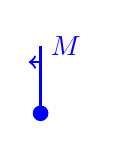
\begin{tikzpicture}[scale=0.5,baseline=0pt]
        \plaquette
        \draw[blue, thick] (0.6,0) node[fill=blue,circle,inner sep=2pt]{};
        \draw[blue, thick] (0.6,0) -- (0.6,1.7)node[above,right]{$M$};
        % --- 上部の青い矢印(左→右)
        \draw[->, blue, thick] (0.6,1.3) -- (0.3,1.3);
        \end{tikzpicture}\ 
        =\ \omega\ 
        \begin{tikzpicture}[scale=0.5,baseline=0pt]
        \plaquette
        \end{tikzpicture}
    \end{align}
\end{itemize}
まとめると、$S(U')$と$S(U)$は$\Sigma$上のみで異なります。つまり、$\Sigma$に局在した欠陥が存在します。作り方からこの欠陥はトポロジカルになります。これを$V_{\omega^{-1}}(\Sigma)$と書くことにします。同様にして$V_{\omega^{n}}(\Sigma)$も定義できます。これらは\SU(N)の中心$\Zcal$の構造を持っています。したがって、1形式対称性の公理をすべて満たすので、1形式対称性になっています。特にこの例の対称性は\kyou{中心対称性}と呼ばれます。

この中心対称性は\kyou{Wilsonループ}に作用します。まず、Wilsonループとは次のような演算子です。$C$をリンクを繋いでいってできる向きのついた閉曲線とします。$C$上のサイトを順に$i_0,i_1,\dots,i_K=i_0$として、基本表現のWilsonループ$W_{\Box}(C)$を
\begin{align}
    W_{\Box}(C) = \Tr\left( U_{i_0 i_1} U_{i_1 i_2} \cdots U_{i_{K-1} i_K}\right)
\end{align}
と定義します。一般に\SU(N)の表現$\rho$に対して、Wilsonループ$W_{\rho}(C)$は
\begin{align}
    W_{\rho}(C) = \Tr\left( \rho(U_{i_0 i_1} U_{i_1 i_2} \cdots U_{i_{K-1} i_K})\right)
\end{align}
と定義します。Wilsonループはゲージ不変な演算子です。

中心対称性のWilsonループへの作用を見るには、次のようにします。Wilsonループ$W_{\Box}(C)$が存在する場合に、$M$として$C$と1回だけ正の向きで交わる余次元1の面をとり、先程の変換を行います。
\begin{align}
    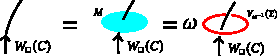
\includegraphics[scale=2]{WTWilsonloop.pdf}
\end{align}
整理すると次のような恒等式が得られます。
\begin{align}
    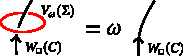
\includegraphics[scale=2]{WTWilsonloop2.pdf}
\end{align}
これは、中心対称性のWard-Takahashi恒等式と呼ぶべきものです。一般のWilsonループ$W_{\rho}(C)$に対しては、Ward-Takahashi恒等式は次のようになります。既約表現$\rho$は基本表現$\ell$個のテンソル積で得られるとします。
\begin{align}
    \underbrace{{
    \Box \otimes \Box \otimes \dots \otimes \Box}_{\ell}} = \rho \oplus \dots
\end{align}
このとき、$\ell \mod{N}$を$\rho$の$N$-alityと呼びます。別の言い方をすると、$\rho$をYoung図で表したときの箱の数を$\mod{N}$で考えたものが$N$-alityです。$\rho$の$N$-alityを$\ell$として、Ward-Takahashi恒等式は
\begin{align}
    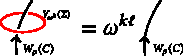
\includegraphics[scale=2]{WTWilsonloop3.pdf}
\end{align}
と書けます。
\section{背景ゲージ場その1}
\ref{sec:backgroundgaugefield}節で見たように、普通の対称性の場合には対称性のトポロジカル欠陥を考えることと、flatな背景ゲージ場を考えることは同じことでした。高次形式対称性の場合も同様に、トポロジカル欠陥を考えることと、背景ゲージ場を考えることは同じことです。
高次形式対称性の場合にも背景ゲージ場の配位としてトポロジカル欠陥を考えることは有用です。この節では格子の場合に$1$形式対称性の背景ゲージ場を考えます。

具体的にするために、格子で$\Zb_N^{(1)}$対称性を考えます。この場合、各プラケット$\expval{ijkl}$に$\Zb_N=\{0,1,\dots,N-1\}$の元$B_{ijkl}$を割り当てます。これを$\Zb_N$ 2形式ゲージ場と呼びます。

$\Zb_N$ 2形式ゲージ場に対するゲージ変換は次のようにします。ゲージ変換のパラメーターは各リンク$\expval{ij}$に割り当てられた$\Zb_N$の元$\Lambda_{ij}$、つまり普通の$\Zb_N$ゲージ場です。ゲージ変換は
\begin{align}
    B_{ijkl}' =& B_{ijkl} + \delta \Lambda_{ijkl},\\
    \delta \Lambda_{ijkl}:=&\Lambda_{ij} + \Lambda_{jk} + \Lambda_{kl} + \Lambda_{li}
    \label{1formgaugetranaf1}
\end{align}
となります。

2形式ゲージ場$B_{ijkl}$に対する場の強さ$\delta B$は、各立方体$c$に割り当てられた$\Zb_N$の元で、次のように定義します。
\begin{align}
    \delta B_c = \sum_{p:\text{立方体の表面の各プラケット}} B_{p}
\end{align}
とします。ただし、$p$の向きは立方体の外側から見て反時計回りになるようにします。このように定義すると、$\delta B_c$はゲージ不変、つまり$\delta \delta \Lambda_c =0$となります。これは、立方体の表面の各リンクは2つのプラケットに共有されていて、それらの相対的な向きが逆になっているため、各リンクからの寄与が打ち消しあうからです。

普通の対称性の場合と同様にすべての$c$で場の強さが$\delta B_c=0$となるようなものをflatな背景ゲージ場と呼びます。flatな背景ゲージ場はゲージ変換をすることで局所的に$B=0$にすることができます。このゲージ変換を繰り返して$B=0$の領域を広げていくと、$B\ne 0$の部分は余次元2の部分(とそのジャンクションなど)に限られます。このような$B\ne 0$の部分がトポロジカル欠陥となります。

次に、この2形式ゲージ場$B$と格子ゲージ理論の結合を考えます。この結合を表す作用は\eqref{Wilsonaction}に$B$を結合させることで、次のように与えられます。
\begin{align}
    S(U,B)=-K\sum_{\expval{ijkl}}\left[ \Tr\left( U_{ij}U_{jk}U_{kl}U_{li}\right) \exp\left(2\pi i B_{ijkl}/N\right)+(\text{複素共役})\right]
    \label{centerbackgroundaction}
\end{align}
とします。この作用は次のようにゲージ対称性を保ちます。$B$のゲージ変換は\eqref{1formgaugetranaf1}です。リンク変数$U$のゲージ変換は
\begin{align}
    U_{ij}' = U_{ij} \exp\left(-2\pi i \Lambda_{ij}/N\right)\label{centergaugetrans2}
\end{align}
とします。この変換で作用\eqref{centerbackgroundaction}は不変であることが分かります。また、中心対称性のトポロジカル欠陥を発見するためにやってみた変換\eqref{centergaugetrans}は、ここで見た\eqref{centergaugetrans2}と同じものであることが分かるでしょう。ここからも中心対称性のトポロジカル欠陥の配位が2形式背景ゲージ場の配位と同じであることが分かります。

ここまでは背景ゲージ場として考えてきましたが、1形式対称性のゲージ化についても少しだけコメントします。普通の対称性の場合と同じように$B$のすべての配位について足し合わせることを1形式対称性の「ゲージ化」と呼びます。$\SU(N)$ゲージ理論の中心対称性をゲージ化すると$\SU(N)/\Zb_N$のゲージ理論が得られます。

\section{背景ゲージ場その2:単体コホモロジー}
ここまでは、格子ゲージ理論での中心対称性を例として高次形式対称性を考えてきました。ただ、一般の曲がった空間などを考えるときに立方格子で格子化できるとは限りません。ここでは、もう少し広い範囲の空間で考えることができるように、\kyou{単体コホモロジー(simplicial cohomology)}というアイデアを導入します。

大まかなアイデアは次のようなものです。flatなゲージ場は局所的に$0$にできますから、$0$の領域を広げていくことにより空間をボールと同じトポロジーを持つ胞に分けることができます。この分割の双対を考えることで、空間を単体に分割することができます。単体は$0$次元の点、$1$次元の線分、$2$次元の三角形、$3$次元の四面体などを一般化したものです。このような単体の分割を\kyou{単体分割}と呼びます。

格子ゲージ理論を考えるときには空間を立方体に分割しましたが、単体分割はこれを立方体の代わりに単体にしたようなものです。今考えたいものはトポロジカルなもので、距離などにはよらないものです。ですから長さは考えなくて良いですし、荒い分割でも問題ありません。このような状況では立方体の格子よりも単体の方が柔軟で応用も効きます。ここでは、単体分割を用いて高次形式対称性を記述することを考えます。

\subsection{Chain}
言葉を導入していきます。$X$をコンパクトで向きのついた多様体とし、この単体分割を$K$とします。この頂点に通し番号$0,1,2,\dots$をふります。この単体分割や通し番号は人為的ですが、この人為的なものによるものか、よらないものかを考えることは重要です。このあたり、ゲージ理論のゲージ固定に似ていますね。

$K$の中の単体をそれに含まれる頂点を用いて表します。例えば頂点($0$単体)はその頂点の番号$i_0$を用いて$\expval{i_0}$、2つの頂点$i_0,i_1$ $(i_0<i_1)$をつなぐ線分($1$単体)は$\expval{i_0 i_1}$、$3$つの頂点$i_0,i_1,i_2$ $(i_0<i_1<i_2)$をつなぐ三角形($2$単体)は$\expval{i_0 i_1 i_2}$と表します。
一般に$p$次元の単体は$p$単体と呼ばれます。
$p+1$個の頂点$i_0,  i_1,\dots,i_p$ $(i_0<i_1<\dots<i_p)$からなる$p$単体を$\expval{i_0,i_1,\dots,i_p}$と表します。
頂点の順番を変えるとどうなるかを考えるとややこしくなるので、\kyou{必ず小さい順に並べることにします。}
以下では、$\expval{i_0,i_1,\dots,i_p}$と添字を書くのが面倒なので$\expval{0\dots p}$の場合を考えても一般性を失わないことを用いて、添字を書く量を減らします。

$G$をアーベル群とします。群演算は$+$で表すことにします。$C_{p}(K,G)$を$K$の中の$p$単体に$G$の元をかけて形式的に和をとったものとします。つまり、$C_{p}(K,G)$は次のように定義されます。
\begin{align}
    C_{p}(K,G) = \{\sum_{\Delta:\ K\text{の$p$単体}} g_{\Delta} \Delta,\quad g_{\Delta}\in G\}
\end{align}
$C_p(K,G)$には係数ごとの足し算によって足し算が定義されます。この足し算により$C_p(K,G)$はアーベル群になります。

次に境界(boudary)演算子
$\del:C_p(K,G)\to C_{p-1}(K,G)$を定義します。これは$p$単体$\expval{0\dots p}$に対して
\begin{align}
    \del \expval{0\dots p} = \expval{12\dots p} - \expval{02\dots p} + 
    =\sum_{i=0}^{p} (-1)^{i} \expval{0\dots \hat{i}\dots p}
\end{align}
と定義します。ここで$\hat{i}$は$i$を抜いたことを表しています。



\section{自発的対称性の破れ}


\end{document}